\documentclass[journal,12pt,twocolumn]{IEEEtran}

\usepackage{setspace}
\usepackage{gensymb}

\singlespacing


\usepackage[cmex10]{amsmath}

\usepackage{amsthm}

\usepackage{mathrsfs}
\usepackage{txfonts}
\usepackage{stfloats}
\usepackage{bm}
\usepackage{cite}
\usepackage{cases}
\usepackage{subfig}

\usepackage{longtable}
\usepackage{multirow}

\usepackage{enumitem}
\usepackage{mathtools}
\usepackage{steinmetz}
\usepackage{tikz}
\usepackage{circuitikz}
\usepackage{verbatim}
\usepackage{tfrupee}
\usepackage[breaklinks=true]{hyperref}
\usepackage{graphicx}
\usepackage{tkz-euclide}
\usepackage{float}

\usetikzlibrary{calc,math}
\usepackage{listings}
    \usepackage{color}                                            %%
    \usepackage{array}                                            %%
    \usepackage{longtable}                                        %%
    \usepackage{calc}                                             %%
    \usepackage{multirow}                                         %%
    \usepackage{hhline}                                           %%
    \usepackage{ifthen}                                           %%
    \usepackage{lscape}     
\usepackage{multicol}
\usepackage{chngcntr}

\DeclareMathOperator*{\Res}{Res}

\renewcommand\thesection{\arabic{section}}
\renewcommand\thesubsection{\thesection.\arabic{subsection}}
\renewcommand\thesubsubsection{\thesubsection.\arabic{subsubsection}}

\renewcommand\thesectiondis{\arabic{section}}
\renewcommand\thesubsectiondis{\thesectiondis.\arabic{subsection}}
\renewcommand\thesubsubsectiondis{\thesubsectiondis.\arabic{subsubsection}}


\hyphenation{op-tical net-works semi-conduc-tor}
\def\inputGnumericTable{}                                 %%

\lstset{
%language=C,
frame=single, 
breaklines=true,
columns=fullflexible
}
\begin{document}
\newtheorem{theorem}{Theorem}[section]
\newtheorem{problem}{Problem}
\newtheorem{proposition}{Proposition}[section]
\newtheorem{lemma}{Lemma}[section]
\newtheorem{corollary}[theorem]{Corollary}
\newtheorem{example}{Example}[section]
\newtheorem{definition}[problem]{Definition}

\newcommand{\BEQA}{\begin{eqnarray}}
\newcommand{\EEQA}{\end{eqnarray}}
\newcommand{\define}{\stackrel{\triangle}{=}}
\bibliographystyle{IEEEtran}
\providecommand{\mbf}{\mathbf}
\providecommand{\pr}[1]{\ensuremath{\Pr\left(#1\right)}}
\providecommand{\qfunc}[1]{\ensuremath{Q\left(#1\right)}}
\providecommand{\sbrak}[1]{\ensuremath{{}\left[#1\right]}}
\providecommand{\lsbrak}[1]{\ensuremath{{}\left[#1\right.}}
\providecommand{\rsbrak}[1]{\ensuremath{{}\left.#1\right]}}
\providecommand{\brak}[1]{\ensuremath{\left(#1\right)}}
\providecommand{\lbrak}[1]{\ensuremath{\left(#1\right.}}
\providecommand{\rbrak}[1]{\ensuremath{\left.#1\right)}}
\providecommand{\cbrak}[1]{\ensuremath{\left\{#1\right\}}}
\providecommand{\lcbrak}[1]{\ensuremath{\left\{#1\right.}}
\providecommand{\rcbrak}[1]{\ensuremath{\left.#1\right\}}}
\theoremstyle{remark}
\newtheorem{rem}{Remark}
\newcommand{\sgn}{\mathop{\mathrm{sgn}}}
\providecommand{\abs}[1]{\left\vert#1\right\vert}
\providecommand{\res}[1]{\Res\displaylimits_{#1}} 
\providecommand{\norm}[1]{\left\lVert#1\right\rVert}
%\providecommand{\norm}[1]{\lVert#1\rVert}
\providecommand{\mtx}[1]{\mathbf{#1}}
\providecommand{\mean}[1]{E\left[ #1 \right]}
\providecommand{\fourier}{\overset{\mathcal{F}}{ \rightleftharpoons}}
%\providecommand{\hilbert}{\overset{\mathcal{H}}{ \rightleftharpoons}}
\providecommand{\system}{\overset{\mathcal{H}}{ \longleftrightarrow}}
	%\newcommand{\solution}[2]{\textbf{Solution:}{#1}}
\newcommand{\solution}{\noindent \textbf{Solution: }}
\newcommand{\cosec}{\,\text{cosec}\,}
\providecommand{\dec}[2]{\ensuremath{\overset{#1}{\underset{#2}{\gtrless}}}}
\newcommand{\myvec}[1]{\ensuremath{\begin{pmatrix}#1\end{pmatrix}}}
\newcommand{\mydet}[1]{\ensuremath{\begin{vmatrix}#1\end{vmatrix}}}
\numberwithin{equation}{subsection}
\makeatletter
\@addtoreset{figure}{problem}
\makeatother
\let\StandardTheFigure\thefigure
\let\vec\mathbf
\renewcommand{\thefigure}{\theproblem}
\def\putbox#1#2#3{\makebox[0in][l]{\makebox[#1][l]{}\raisebox{\baselineskip}[0in][0in]{\raisebox{#2}[0in][0in]{#3}}}}
     \def\rightbox#1{\makebox[0in][r]{#1}}
     \def\centbox#1{\makebox[0in]{#1}}
     \def\topbox#1{\raisebox{-\baselineskip}[0in][0in]{#1}}
     \def\midbox#1{\raisebox{-0.5\baselineskip}[0in][0in]{#1}}
\vspace{3cm}
\title{ASSIGNMENT4}
\author{SOWMYA BANDI}
\maketitle
\newpage
\bigskip
\renewcommand{\thefigure}{\theenumi}
\renewcommand{\thetable}{\theenumi}
Download all python codes from 
\begin{lstlisting}
https://github.com/Sowmyabandi99/Assignment3/tree/main/Assignment3/Assignment3
\end{lstlisting}
%
and download all latex-tikz codes from 
%
\begin{lstlisting}
https://github.com/CRAMYATULASI/ASSIGNMENT5/tree/main/ASSIGNMENT5
\end{lstlisting}
%
\section{Question No 2.40}
Find the equation of the plane passing through the intersection of the planes 
\begin{align}
\myvec{2 & 2 & -3}\vec{x}&=7 \label{eq1}
\\
\myvec{2 & 5 & 3}\vec{x}&=9 \label{eq2}
\end{align}
%
and the point $\myvec{2\\ 1 \\ 3}$ \label{eq3}

\section{SOLUTION} 
The intersection of the planes is obtained by row reducing the augmented  matrix as 
\begin{align}
\myvec{2 & 2 & -3 & 7\\2 & 5 & 3 & 9} 
\xleftrightarrow{R_1\leftarrow \frac{R_1}{2}}\myvec{1 & 1 & \frac{-3}{2} & \frac{7}{2}\\2 & 5 & 3 & 9} 
\\
%\myvec{1 & 1 & \frac{-3}{2} &\frac{7}{2} \\0 & 3 & 6 & 2}
\xleftrightarrow{R_2\leftarrow R_2 - 2R_1}\myvec{1 & 1 & \frac{-3}{2} &\frac{7}{2} \\0 & 3 & 6 & 2}
\\
%\myvec{1 & 1 & \frac{-3}{2} & \frac{7}{2}\\0 & 1 & 2 & \frac{2}{3}}
\xleftrightarrow{R_2\leftarrow \frac{R_2}{3}}\myvec{1 & 1 & \frac{-3}{2} & \frac{7}{2}\\0 & 1 & 2 & \frac{2}{3}}
\\
%\myvec{1 & 0 & \frac{-7}{2} & \frac{17}{6}\\0 & 1 & 2 & \frac{2}{3}}
\xleftrightarrow{R_1\leftarrow R_1 - R_2}\myvec{1 & 0 & \frac{-7}{2} & \frac{17}{6}\\0 & 1 & 2 & \frac{2}{3}}
\\
\implies\vec{x}=\myvec{\frac{17}{6} \\ \frac{2}{3} \\ 0}+\lambda\myvec{\frac{7}{2} \\ -2 \\ 1}   \label{eq4}
\end{align}
Thus, $\myvec{\frac{17}{6} \\ \frac{2}{3} \\ 0}$ is another point on the plane.The normal vector to the plane is then obtained as 
\begin{align}
\myvec{\myvec{2 \\ 1 \\ 3}-\myvec{\frac{17}{6} \\ \frac{2}{3} \\ 0}}\myvec{\frac{7}{2} \\ -2 \\ 1}
\end{align}
which can be obtained by row reducing the matrix
\begin{align}
\myvec{\frac{7}{2} & -2 & 1\\\frac{-5}{6} & \frac{1}{3} & 3} 
\xleftrightarrow{R_1\leftarrow \ \frac{2}{7}R_1}\myvec{1 & \frac{-4}{7} & \frac{2}{7}\\\frac{-5}{6} & \frac{1}{3} & 3} 
\\
%\myvec{1 & \frac{-4}{7} & \frac{2}{7}\\0 & \frac{-1}{7} & \frac{68}{21}}
\xleftrightarrow{R_2\leftarrow R_2 + \frac{5}{6}R_1}\myvec{1 & \frac{-4}{7} & \frac{2}{7}\\0 & \frac{-1}{7} & \frac{68}{21}}
\\
%\myvec{1 & 0 & \frac{-38}{3}\\0 & \frac{-1}{7} & \frac{68}{21}}
\xleftrightarrow{R_1\leftarrow R_1 - 4R_2}\myvec{1 & 0 & \frac{-38}{3} \\ 0 & \frac{-1}{7} & \frac{68}{21}}
\\
\implies\vec{n}=\myvec{\frac{38}{3} \\ \frac{68}{3} \\ 1}=\myvec{38\\68\\3}   \label{eq5}
\end{align}
Since the plane passing through $\myvec{2\\1\\3}$, using \eqref{eq5}
\begin{align}
\myvec{38 & 68 & 3}\myvec{\vec{x}-\myvec{2 \\ 1 \\ 3}}=0
\\
\implies\myvec{38 & 68 & 3}\vec{x}=153
\end{align}
Alternatively,the plane passing through the intersection of \eqref{eq1} and \eqref{eq2} has the form 
\begin{align}
\myvec{2 & 2 & -3}\vec{x}+\lambda\myvec{2 & 5 & 3}\vec{x}=7+9\lambda
\end{align}
substituting \myvec{2 \\ 1 \\ 3} in the above,
\begin{align}
\myvec{2 & 2 & -3}\myvec{2 \\ 1 \\ 3}+\lambda\myvec{2 & 5 & 3}\myvec{2 \\ 1 \\ 3}&=7+9\lambda   \label{eq6}
\\
\implies -3+18\lambda&=7+9\lambda
\\
\implies \lambda&=\frac{10}{9}
\end{align}
substituting value of $\lambda$ in \eqref{eq6} yields the equation of the plane.
\begin{align}
\myvec{38 & 38 & 3}\vec{x}=153
\end{align}
Plot of the plane 
\numberwithin{figure}{section}
\begin{figure}[ht]
\centering
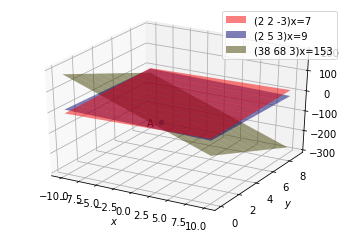
\includegraphics[width=\columnwidth]{Figure.png}
\caption{Plot of the plane}
\label{Plot of the plane}
\end{figure}
\end{document}
